\chapter{Implementasi, Eksperimen, dan Hasil Evaluasi Eksperimen}

Bab ini menjelaskan proses implementasi dari rancangan solusi yang telah dikaji pada Bab \ref{sec:chapter-3} dalam menyelesaikan permasalahan utama tugas akhir, yaitu pemanfaatan berbagai metode PEFT pada kakas evaluasi IndoLEM. Selain itu, dijelaskan juga lingkungan, implementasi, dan eksperimen. Lingkungan untuk implementasi dan eksperimen dibedakan, lingkungan eksperimen dijelaskan pada subbab \ref{sec:lingkungan-eksperimen}, sedangkan lingkungan implementasi dijelaskan pada subbab \ref{sec:pengembangan-kakas}.

Berdasarkan rancangan solusi yang diajukan pada subbab \ref{sec:rancangan-solusi}, pembangunan ulang kakas IndoLEM diperlukan untuk mengimplementasi setiap metode PEFT. Model yang dipilih adalah IndoBERT untuk tugas evaluasi \textit{classification} dan IndoT5 untuk tugas evaluasi \textit{generation} dilatih pada lingkungan eksperimen. Model yang telah dilatih dengan metode \textit{fine-tuning}  dan metode PEFT dievaluasi untuk membandingkan kinerja dari setiap metode pada setiap tugas evaluasinya.

\section{Lingkungan}
\section{Pengembangan Ulang Kakas IndoLEM}
\label{sec:pengembangan-kakas}

Pengembangan ulang kakas IndoLEM ini diperlukan untuk memperbarui dan memperbaiki infrastruktur dari kakas tersebut. Pengembangan ini dilakukan pada lingkungan lokal pribadi, untuk keperluan eksperimen dilakukan pada lingkungan \textit{cloud} seperti yang sudah disebutkan pada subbab \ref{sec:lingkungan-eksperimen}.

\subsection{Persiapan Lingkungan Pengembangan}

Implementasi diawali dengan menyiapkan lingkungan pengembangan, untuk menyiapkan lingkungan pengembangan dilakukan dengan melakukan instalasi terhadap perangkat lunak dan pustaka yang dibutuhkan. Berikut merupakan \textit{requirements.txt} yang berisi pustaka yang perlu dilakukan intalasi yang bisa dilihat pada tabel \ref{table:requirements}

\begin{table}[h]
    \caption{Tabel \textit{requirements.txt}}
    \label{table:requirements}
    \begin{lstlisting}[language=bash]
    accelerate
    adapters==0.2.2
    datasets
    evaluate
    huggingface-hub
    numpy
    pandas
    scikit-learn
    seqeval
    torch
    transformers==4.40.*
    wandb
    nltk
    rouge_score
    indobenchmark-toolkit
    \end{lstlisting}
\end{table}

Untuk memudahkan pengembangan perlu membuat \textit{virtual environment} untuk mengenkapsulasi pustaka yang dipakai. \textit{Virtual environment} bisa dibuat dengan menggunakan Conda atau pustaka virtualenv. Untuk tugas akhir ini, digunakan Conda. \textit{Command} yang digunakan dapat dilihat pada tabel \ref{table:command-virtualenv}.

\begin{table}[h]
    \caption{Tabel \textit{command virtual environment}}
    \label{table:command-virtualenv}
    \begin{lstlisting}[language=bash]
    # Membuat virtual environment
    conda create env -n indolem python=3.11
    # Menjalankan virtual environment
    conda activate indolem
    # Melakukan instalasi pustaka 
    pip install -r requirements.txt
    \end{lstlisting}
\end{table}

\textit{Command} tersebut akan membuat \textit{virtual environment}, mengakitfkannya, dan melakukan instalasi pada versi Python dan pustaka yang dibutuhkan.

\subsection{Penguraian Argumen}
\label{sec:parse-arg}

Penguraian argumen dilakukan dengan menggunakan modul HfArgumentParser dari pustaka Transformers. Modul ini digunakan untuk memudahkan penguraian argumen karena argumen yang dipakai untuk model, pelatihan, dan evaluasi sudah diimplementasikan dari modul tersebut. Untuk argumen tambahan yang spesifik pada suatu tugas evaluasi perlu ditambahkan secara manual, sebagai contoh pada tugas evaluasi NER terdapat argumen \textit{return\_entity\_level\_metrics} yaitu menggunakan metriks evaluasi untuk level entitasnya.

\begin{table}[h]
    \caption{Tabel kode HfArgumentParser}
    \label{table:hfargumentparser}
    \begin{lstlisting}[language=python]
    parser = HfArgumentParser(
        [
            ModelArguments,
            DataTrainingArguments,
            TrainingArguments,
            AdapterArguments,
            WandbArguments,
        ]
    )

    if len(sys.argv) == 2 and sys.argv[1].endswith(".json"):
        # If we pass only one argument to the script and it's the path to a json file,
        # let's parse it to get our arguments.
        model_args, data_args, training_args, adapter_args, wandb_args = (
            parser.parse_json_file(json_file=os.path.abspath(sys.argv[1]))
        )
    else:
        model_args, data_args, training_args, adapter_args, wandb_args = (
            parser.parse_args_into_dataclasses()
        )
    \end{lstlisting}
\end{table}

Berdasarkan tabel \ref{table:hfargumentparser} terdapat 5 jenis argumen, yaitu model, \textit{data training}, pelatihan, \textit{adapter}, dan wandb. Argumen model digunakan untuk pemuatan model. Argumen \textit{data training} digunakan untuk pemuatan \textit{file} (latih, evaluasi, dan uji), \textit{padding}, maksimum sampel, maksimum sekuens, dan lain sebagainya yang berhubungan dengan \textit{dataset}. Lalu, argumen pelatihan merupakan \textit{hyperparemeter} yang digunakan pada proses pelatihan seperti \textit{learning rate, epoch, batch size}, dan lain sebagainya. Selanjutnya, argumen \textit{adapter} berfungsi sebagai konfigurasi untuk jenis metode PEFT beserta \textit{hyperparameter} yang digunakannya. Terakhir, merupakan argumen wandb yang digunakan untuk konfigurasi sinkronisasi pada hasil evaluasi ke \textit{cloud}.

\subsection{Praproses \textit{Dataset}}
\label{sec:praproses}

Praproses \textit{dataset} diperlukan agar model dapat memproses \textit{dataset} dengan konteks yang sesuai. Konteks yang dimaksud adalah, model dapat memahami \textit{metadata} dari \textit{dataset}, sehingga mampu mengetahui setiap bagian data yang merupakan bagian dari teks atau label. Praproses \textit{dataset} ini berbeda untuk setiap tugas evaluasi karena karakteristik dari tugas evaluasinya yang berbeda juga.

\subsubsection{Praproses Data NER}

Tugas evaluasi NER merupakan jenis tugas \textit{classification} pada level token yang berarti setiap token akan diklasifikasikan dengan label tertentu. Pada kakas IndoLEM, untuk tugas evaluasi NER terdapat dua jenis \textit{dataset}, yaitu NERUI dan NERUGM. Kedua \textit{dataset} tersebut mempunyai label yang berbeda berikut merupakan label pada setiap \textit{dataset}-nya dapat dilihat pada tabel \ref{table:label-ner}.

\begin{table}[h]
    \vspace{0.25cm}
    \caption{Tabel label \textit{dataset} NER}
    \label{table:label-ner}
    \begin{center}
        \begin{tabular}{|l|l|}
            \hline \rowcolor{black!10}
            \multicolumn{1}{|c|}{\textbf{NERUI}} & \multicolumn{1}{|c|}{\textbf{NERUI}} \\ \hline
            B-LOCATION & B-LOCATION \\ \hline
            B-ORGANIZATION & B-ORGANIZATION \\ \hline
            B-PERSON & B-PERSON \\ \hline
            - & B-QUANTITY \\ \hline
            - & B-TIME \\ \hline
            I-LOCATION & I-LOCATION \\ \hline
            I-ORGANIZATION & I-ORGANIZATION \\ \hline
            I-PERSON & I-PERSON \\ \hline
            - & I-QUANTITY \\ \hline
            - & I-TIME \\ \hline
            O & O \\ \hline
        \end{tabular}
    \end{center}
\end{table}

Label tersebut diperlukan untuk melakukan \textit{mapping} antara id dengan labelnya yang akan digunakan pada konfigurasi model. \textit{Padding} juga dilakukan berdasarkan panjang sekuens maksimum yang didefinisikan melaluai argumen \textit{data training}. Selanjutnya, tokenisasi akan dilakukan terhadap \textit{dataset} tersebut. Implementasi dari fungsi tokenisasi tersebut dapat dilihat pada tabel \ref{table:tokenisasi-ner}.

\begin{table}[h]
    \caption{Tabel fungsi tokenisasi NER}
    \label{table:tokenisasi-ner}
    \begin{lstlisting}[language=python]
    def tokenize_and_align_labels(examples):
        tokenized_inputs = tokenizer(
            examples[text_column_name],
            padding=padding,
            truncation=True,
            max_length=data_args.max_seq_length,
            is_split_into_words=True,
        )
        labels = []

        for i, label in enumerate(examples[label_column_name]):
            word_ids = tokenized_inputs.word_ids(batch_index=i)
            previous_word_idx = None
            label_ids = []
            for word_idx in word_ids:
                if word_idx is None:
                    label_ids.append(-100)
                elif word_idx != previous_word_idx:
                    label_ids.append(label_to_id[label[word_idx]])
                else:
                    if data_args.label_all_tokens:
                        label_ids.append(b_to_i_label[label_to_id[label[word_idx]]])
                    else:
                        label_ids.append(-100)
                previous_word_idx = word_idx

            labels.append(label_ids)
        tokenized_inputs["labels"] = labels
        return tokenized_inputs
    \end{lstlisting}
\end{table}

Tokenisasi dilakukan dengan menggunakan modul Tokenizer pada pustaka Transformers. Fungsi tokenisasi pada tabel \ref{table:tokenisasi-ner} mengabaikan token spesial [CLS] dan [SEP] yang muncul dari hasil tokenisasi model berbasi BERT. Token spesial tersebut diubah menjadi -100 agar bisa diabaikan dari perhitungan metriks evaluasinya. Sehingga, hanya token yang berkorespondensi terhadap sebuah label saja yang dapat dievaluasi.

\subsubsection{Praproses Data \textit{Sentiment Analysis}}

Tugas evaluasi \textit{sentiment analysis} merupakan jenis tugas \textit{classification} sama seperti NER, hanya perbedaannya pada level klasifikasi yang digunakan. Jika pada NER klasifikasi dilakukan pada level token, pada \textit{sentiment analysis} klasifikasi dilakukan pada level teks yang merupakan gabungan dari beberapa token. \textit{Dataset} dari \textit{sentiment analysis} berupa \textit{file} CSV yang berisi dari dua kolom yaitu \textit{sentence} dan \textit{labels}. Kolom \textit{sentence} merupakan teks yang mengandung sentiment tertentu. Sementara kolom \textit{labels} menandakan sentimen dari teks tersebut, dengan nilai 0 berupa sentimen negatif dan  nilai 1 berupa sentiment positif.

\begin{table}[h]
    \caption{Tabel fungsi tokenisasi \textit{sentiment analysis}}
    \label{table:tokenisasi-sentiment}
    \begin{lstlisting}[language=python]
        def preprocess_function(examples):
            # Tokenize the texts
            args = (
                (examples[sentence1_key],)
                if sentence2_key is None
                else (examples[sentence1_key], examples[sentence2_key])
            )
            result = tokenizer(
                *args, padding=padding, max_length=max_seq_length, truncation=True
            )

            # Map labels to IDs
            if label_to_id is not None and "labels" in examples:
                result["labels"] = [
                    (label_to_id[l] if l != -1 else -1) for l in examples["labels"]
                ]
            return result
    \end{lstlisting}
\end{table}

Pada tugas evaluasi \textit{sentiment analysis} juga diperlukan \textit{mapping} antara label dengan idnya, sehingga model mampu mengetahui label yang dilatih. Fungsi tokenisasi \textit{sentiment analysis} yang dapat dilihat pada tabel \ref{table:tokenisasi-sentiment} menggunakan modul Tokenizer dari pustaka Transformers. Fungsi tersebut terdapat \textit{sentence1\_key} dan juga \textit{sentence2\_key}, yang berguna apabila terdapat dua kolom teks pada \textit{dataset}, tetapi pada IndoLEM \textit{dataset sentiment analysis} hanya mempunyai satu kolom teks. Sehingga, \textit{sentence2\_key} tidak digunakan. 

\subsubsection{Praproses Data \textit{Summarization}}

Tugas evaluasi \textit{summarization} merupakan jenis tugas \textit{generation} yang berbeda dengan jenis tugas \textit{classification}. Tugas \textit{generation} memerlukan generasi teks untuk dapat dilakukan evaluasi, pada konteks ini yaitu membuat ringkasan dari teks. \textit{Dataset} yang digunakan pada IndoLEM untuk tugas evaluasi \textit{summarization} adalah \textit{dataset} IndoSUM. \textit{Dataset} ini berisi \textit{file} dengan format JSONL dengan masing-masing objek dapat dilihat pada tabel \ref{table:data-summarization}.

\begin{table}[h]
    \vspace{0.25cm}
    \caption{Tabel data \textit{summarization}}
    \label{table:data-summarization}
    \begin{center}
        \begin{tabular}{|l|l|}
            \hline \rowcolor{black!10}
            \multicolumn{1}{|c|}{\textbf{Objek}} & \multicolumn{1}{|c|}{\textbf{Deskripsi}} \\ \hline
            id & nilai unik untuk setiap artikel \\ \hline
            paragraphs & \textit{list} dari paragraf yang berasal dari artikel \\ \hline
            summary & ringkasan dari artikel, disimpan sebagai \textit{list} dari kalimat \\ \hline 
            gold\_labels & label ekstraktif dari setiap kalimat pada artikel \\ \hline
            category & kategori dari artikel \\ \hline
            source & sumber artikel \\ \hline
            source\_url & URL dari artikel \\ \hline
        \end{tabular}
    \end{center}
\end{table}

Dari data yang dapat dilihat pada tabel \ref{table:data-summarization}, terdapat 7 objek  pada \textit{dataset}. Namun, pada tugas evaluasi ini hanya akan digunakan dua objek yaitu \textit{paragraphs} dan \textit{summary} karena tugas \textit{summarization} membutuhkan teks asli sebelum diringkas dan hasil ringkasannya. Objek yang lain selain dua yang digunakan bisa diabaikan saja. \textit{Dataset} ini perlu dipraproses terlebih dahulu menggunakan fungsi yang dapat dilihat pada tabel \ref{table:tokensisasi-summ}.

\begin{table}[h]
    \caption{Tabel fungsi tokenisasi \textit{summarization}}
    \label{table:tokensisasi-summ}
    \begin{lstlisting}[language=python]
    def preprocess_function(examples):
        if is_indosum:
            examples[text_column] = paragraph_to_text(examples[text_column])
            examples[summary_column] = summary_to_text(examples[summary_column])

        inputs = [prefix + inp for inp in inputs]
        model_inputs = tokenizer(
            inputs,
            max_length=data_args.max_source_length,
            padding=padding,
            truncation=True,
        )

        labels = tokenizer(
            text_target=targets,
            max_length=max_target_length,
            padding=padding,
            truncation=True,
        )

        if padding == "max_length" and data_args.ignore_pad_token_for_loss:
            labels["input_ids"] = [
                [(l if l != tokenizer.pad_token_id else -100) for l in label]
                for label in labels["input_ids"]
            ]

        model_inputs["labels"] = labels["input_ids"]
        return model_inputs
    \end{lstlisting}
\end{table}

Berdasarkan tabel \ref{table:tokensisasi-summ}, tokenisasi dilakukan dengan mengolah objek \textit{paragraphs} menjadi \textit{list} dari teks. Setiap paragraf terdiri dari beberapa kalimat, dan setiap kalimat terdiri dari beberapa teks. Untuk \textit{text\_column} yang merupakan objek \textit{paragraphs} akan diolah menjadi \textit{list} dari teks. Hal yang sama berlaku juga untuk \textit{summary\_column}, hanya saja objek ini merupakan \textit{summary} yang berisi kalimat. Selain itu, tugas evaluasi \textit{summarization} ini terdapat \textit{prefix} yang berguna pada beberapa model tertentu. Tokenisasi juga menggunakan modul \textit{tokenizer} dari pustaka Transformers.

\subsection{Pemuatan Konfigurasi Model}

Untuk dapat melakukan pelatihan dan evaluasi terhadap model, terlebih dahulu model perlu dimuat. Pemuatan model ini menggunakan konfigurasi yang dimuat dari penguraian argumen pada subbab \ref{sec:parse-arg}. Argumen model akan dimuat ke dalam model sehingga model bisa dipakai. Model akan dimuat dengan menggunakan modul yang relevan dari pustaka Transformers.

\begin{table}[h]
    \caption{Tabel kode pemuatan model \textit{summarization}}
    \label{table:kode-model-summ}
    \begin{lstlisting}[language=python]
    model = AutoModelForSeq2SeqLM.from_pretrained(
        model_args.model_name_or_path,
        from_tf=bool(".ckpt" in model_args.model_name_or_path),
        config=config,
        cache_dir=model_args.cache_dir,
        revision=model_args.model_revision,
        token=True if model_args.token else None,
    )
    \end{lstlisting}
\end{table}

Pada tabel \ref{table:kode-model-summ} dimuat model AutoModelForSeq2SeqLM yang merupakan model \textit{sequence to sequence} yang merupakan model \textit{encoder decoder}. Modul AutoModel ini akan menghasilkan model berdasarkan dari konfigurasi \textit{model\_args} yang dimasukkan pada modul tersebut. Untuk tugas evaluasi \textit{summarization} yang menggunakan model IndoT5 akan menghasilkan model tersebut juga. Berbeda untuk tugas \textit{classification}, cukup dengan menyatakan AutoModel saja sudah cukup untuk menghasilkan model yang sesuai. Pada konteks ini, model yang digunakan untuk NER dan \textit{sentiment analysis} adalah IndoBERT yang berbasis BERT.

\subsection{Perhitungan Metriks Evaluasi}
\label{sec:metriks-evaluasi}

Metriks evaluasi yang digunakan pada setiap tugas evaluasi tidak sama semuanya. Metriks yang digunakan untuk tugas \textit{classification} adalah \textit{accuracy} dan F1 \textit{score}. Sedangkan, pada tugas \textit{generation} adalah ROUGE \textit{score}. Perhitungan metriks evaluasi ini dilakukan saat proses evaluasi dengan menggunakan fungsi \textit{compute\_metrics}.

\begin{table}[h]
    \caption{Tabel fungsi \textit{compute\_metrics}}
    \label{table:compute-metrics}
    \begin{lstlisting}[language=python]
    def compute_metrics(p):
        logits, labels = p
        predictions = np.argmax(logits, axis=1)

        return {
            "accuracy": accuracy_score(labels, predictions),
            "precision": precision_score(labels, predictions, average="macro"),
            "recall": recall_score(labels, predictions, average="macro"),
            "f1": f1_score(labels, predictions, average="macro"),
        }
    \end{lstlisting}
\end{table}

Pada tabel \ref{table:compute-metrics}, fungsi perhitungan metriks evaluasinya merupakan fungsi yang dipakai untuk tugas \textit{classification}. Fungsi tersebut memanfaatkan modul seqeval untuk melakukan perhitungan setiap metriksnya. Terdapat perbeedaan pada fungsi yang dipakai pada tugas \textit{classifcation}, NER menggunakan \textit{entity\_level\_metrics} yang berarti perhitungan evaluasinya berdasarkan pada entitasnya yang berbeda dengan \textit{sentiment analysis}. Untuk tugas \textit{generation} yaitu \textit{summarization} menggunakan ROUGE \textit{score}.

\subsection{Pemuatan Trainer untuk Pelatihan dan Evaluasi Model}

Untuk pelatihan dan evaluasi model dibutuhkan standardisasi agar kode yang digunakan pada setiap tugas tidak berbeda. Modul Trainer dari pustaka Transformers digunakan untuk pelatihan dan evaluasi model. Setiap komponen yang sudah disebutkan sebelumnya akan dimuat pada modul Trainer. Setiap tugas evaluasi akan menggunakan implementasi yang sama yang bisa dilihat pada tabel \ref{table:kode-trainer}.

\begin{table}[h]
    \caption{Tabel kode implementasi Trainer}
    \label{table:kode-trainer}
    \begin{lstlisting}[language=python]
    trainer = Trainer(
        model=model,
        args=training_args,
        train_dataset=train_dataset if training_args.do_train else None,
        eval_dataset=eval_dataset if training_args.do_eval else None,
        tokenizer=tokenizer,
        data_collator=data_collator,
        compute_metrics=compute_metrics,
    )

    trainer.train(resume_from_checkpoint=checkpoint)
    trainer.evaluate()
    \end{lstlisting}
\end{table}

Kode implementasi Trainer pada tabel \ref{table:kode-trainer} memuat modul Trainer dan memanggil metode \textit{train} dan \textit{evaluate} untuk melakukan pelatihan dan evaluasi. Modul Trainer membutuhkan beberapa argumen yang dimuat. Argumen tersebut dimuat dari komponen-komponen yang sudah disebutkan pada subbab sebelumnya. Argumen untuk pelatihan, dan model didapat dari hasil penguraian argumen pada \ref{sec:parse-arg}. Untuk \textit{tokenizer} dan \textit{dataset} pelatihan dan evaluasi dimuat dari hasil praproses data pada \ref{sec:praproses}. Lalu, untuk \textit{compute\_metrics} fungsinya dimuat dari metriks evaluasi pada \ref{sec:metriks-evaluasi}. 

\section{Pengembangan Metode PEFT pada Kakas IndoLEM}

Pengembangan metode PEFT pada kakas IndoLEM menggunakan pustaka Adapters. Pustaka tersebut tidak hanya mengimplementasikan setiap metode saja, tetapi terdapat fungsionalitas untuk menggabungkan beberapa metode PEFT. Pada subbab sebelumnya yaitu subbab \ref{sec:pengembangan-kakas}, kakas IndoLEM dikembangkan ulang agar mampu untuk mengimplementasikan metode PEFT. Implementasi tersebut  mengubah beberapa komponen, yaitu komponen model dan trainer. Metode PEFT  melakukan \textit{freeze} pada parameter model sehingga pada proses pelatihan tidak  mengubah parameter model melainkan parameter dari metode PEFT tersebut.

\begin{table}[h]
    \caption{Tabel kode pemuatan model Adapters}
    \label{table:kode-model-adapters}
    \begin{lstlisting}[language=python]
    model = AutoAdapterModel.from_pretrained(
        model_args.model_name_or_path,
        from_tf=bool(".ckpt" in model_args.model_name_or_path),
        config=config,
        cache_dir=model_args.cache_dir,
        revision=model_args.model_revision,
        token=True if model_args.token else None,
        ignore_mismatched_sizes=model_args.ignore_mismatched_sizes,
    )
    \end{lstlisting}
\end{table}

Pada kode pemuatan model Adapters yang bisa dilihat pada tabel \ref{table:kode-model-adapters}, model dimuat dengan modul AutoAdapterModel dari pustaka Adapters. Hal ini dilakukan untuk \textit{support} metode PEFT yang lebih baik berdasarkan dari dokumentasi dari pustakanya. Berbeda dari tabel \ref{table:kode-model-summ} yang menggunakan AutoModel dari pustaka Transformers, AutoAdapterModel memberikan fungsionalitas yang lebih baik untuk metode PEFT, salah satunya adalah untuk membandingkan parameter yang  dilatih dibanding dengan parameter asli dari modelnya.

\begin{table}[h]
    \caption{Tabel kode implementasi AdapterTrainer}
    \label{table:kode-adaptertrainer}
    \begin{lstlisting}[language=python]
    setup_adapter_training(model, adapter_args)
    trainer = AdapterTrainer(
        model=model,
        args=training_args,
        train_dataset=train_dataset if training_args.do_train else None,
        eval_dataset=eval_dataset if training_args.do_eval else None,
        tokenizer=tokenizer,
        data_collator=data_collator,
        compute_metrics=compute_metrics,
    )

    trainer.train(resume_from_checkpoint=checkpoint)
    trainer.evaluate()
    \end{lstlisting}
\end{table}

Selanjutnya, untuk proses pelatihan perlu disiapkan untuk menggunakan metode PEFT. Implementasinya menggunakan modul AdapterTrainer dari pustaka Adapters juga. Model perlu disiapkan untuk pelatihan dengan metode PEFT dengan menggunakan fungsi \textit{setup\_adapter\_training}. Fungsi tersebut  melakukan \textit{freeze} pada parameter model dan hanya  mengubah parameter dari metode PEFT yang digunakan. Argumen untuk \textit{adapter} dimuat dari hasil pengurain argumen pada \ref{sec:parse-arg}, argumen tersebut berisi jenis metode PEFT serta \textit{hyperparameter} yang digunakan pada proses pelatihan. Proses pelatihan metode PEFT berbeda dengan pelatihan dengan metode \textit{fine-tuning} tergantung dari karakteristik dari metode tersebut. Pustaka Adapters mengimplementasikannya dengan menambahkan semacam \textit{adapter} pada model, sehingga \textit{adapter} tersebut yang dilatih bukan modelnya. Parameter dari \textit{adapter} tersebut relatif lebih kecil daripada parameter model.

\section{Pelatihan Model}

Pelatihan model dilakukan pada lingkungan eksperimen yang telah disebutkan pada subbab \ref{sec:lingkungan-eksperimen}. Pelatihan dilakukan dengan \textit{bash script} yang  dijalankan pada \textit{shell} untuk memudahkan reka ulang dari eksperimen tersebut. Untuk setiap tugas evaluasi terdapat \textit{bash script} yang  menjalankan semua eksperimen, yaitu \textit{fine-tuning}, \methodPEFT.

\begin{figure}[h]
    \centering
    \caption{Struktur \textit{file} eksperimen}
    \label{fig:file-eksperimen}
    \begin{forest}
        for tree={
            font=\ttfamily,
            grow'=0,
            child anchor=west,
            parent anchor=south,
            anchor=west,
            calign=first,
            edge path={
                \noexpand\path [draw, \forestoption{edge}]
                (!u.south west) +(7.5pt,0) |- node[fill,inner sep=1.25pt] {} (.child anchor)\forestoption{edge label};
            },
            before typesetting nodes={
                if n=1
                    {insert before={[,phantom]}}
                    {}
            },
            fit=band,
            before computing xy={l=15pt},
        }
    [run\_sentiment.sh
        [script
            [run\_sentiment\_base.sh]
            [run\_sentiment\_lora.sh]
            [run\_sentiment\_pt.sh]
            [run\_sentiment\_seq\_bn.sh]
            [run\_sentiment\_unipelt.sh]
        ]
    ]
    \end{forest}
\end{figure}

Pada gambar \ref{fig:file-eksperimen}, dengan melakukan pemanggilan pada {\ttfamily run\_sentiment.sh}  menjalankan semua eksperimen yang ada pada folder {\ttfamily script}. Setiap \textit{script}  menjalankan eksperimen sesuai dari konfigurasi yang telah ditentukan pada \textit{script} tersebut. Konfigurasi yang ditentukan tersebut  diterima sebagai argumen pada kakas IndoLEM. Untuk setiap \textit{hyperparameter} yang digunakan untuk pelatihan dapat dilihat pada tabel \ref{table:hyperparameter-train}.

\begin{table}[h]
    \centering
    \caption{Tabel \textit{hyperparameter} pelatihan}
    \label{table:hyperparameter-train}
    \begin{tabular}{|c|l|c|}
        \hline \rowcolor{black!10}
        \textbf{Tugas} & \multicolumn{1}{|c|}{\textbf{Argumen}} & \textbf{Nilai} \\ \hline
        \multirow{9}{*}{\textit{NER}} & model & "indolem/indobert-base-uncased" \\ \cline{2-3}
                                      & train batch size & 16 \\ \cline{2-3}
                                      & eval batch size & 64 \\ \cline{2-3}
                                      & epochs & 100 \\ \cline{2-3}
                                      & learning rate & 5e-5 \\ \cline{2-3}
                                      & max sequence length & 128 \\ \cline{2-3}
                                      & text column names & "tokens" \\ \cline{2-3}
                                      & label column names & "ner\_tags" \\ \cline{2-3}
                                      & return entity level metrics & true \\ \cline{2-3}
                                      & seed & 42 \\ \hline
        \multirow{7}{*}{\textit{sentiment analysis}} & model & "indolem/indobert-base-uncased" \\ \cline{2-3}
                                                     & batch size & 30 \\ \cline{2-3}
                                                     & epochs & 20 \\ \cline{2-3}
                                                     & learning rate & 5e-5 \\ \cline{2-3}
                                                     & max sequence length & 200 \\ \cline{2-3}
                                                     & seed & 42 \\ \cline{2-3}
                                                     & label names & "labels" \\ \hline
        \multirow{14}{*}{\textit{summarization}} & model & "LazarusNLP/IndoNanoT5-base" \\ \cline{2-3}
                                                & train batch size & 4 \\ \cline{2-3}
                                                & eval batch size & 8 \\ \cline{2-3}
                                                & epochs & 5 \\ \cline{2-3}
                                                & learning rate & 1e-5 \\ \cline{2-3}
                                                & max source length & 512 \\ \cline{2-3}
                                                & max target length & 512 \\ \cline{2-3}
                                                & num beams & 5 \\ \cline{2-3}
                                                & weight decay & 0.01 \\ \cline{2-3}
                                                & patience & 5 \\ \cline{2-3}
                                                & seed & 42 \\ \cline{2-3}
                                                & text column & paragraphs \\ \cline{2-3}
                                                & summary column & summary \\ \cline{2-3}
                                                & source prefix & "summarize: " \\ \cline{2-3}
                                                & pad to max length & true \\ \cline{2-3}
                                                & predict with generate & true \\ \cline{2-3}
                                                & bf16 & true \\ \hline
    \end{tabular}
\end{table}

Untuk pelatihan model NER terdapat dua \textit{dataset} yang  digunakan yaitu NERUGM dan NERUI. Sedangkan, untuk tugas \textit{sentiment analysis} dan \textit{summarization} menggunakan satu dataset. Selain itu, untuk tugas NER terdapat argumen "return entity level metrics" dengan nilai "true" yang berarti penilaian metriks evaluasinya  dinilai pada level entitas. Ini mengikuti eksperimen yang sebelumnya sudah dilakukan pada IndoLEM.

Terdapat perbedaan pada \textit{hyperparameter} yang digunakan untuk tugas \textit{summarization} karena argumen yang digunakan mengikuti eksperimen pada IndoT5 bukan pada IndoLEM. Terdapat juga argumen "predict with generate" dengan nilai "true" karena tugas \textit{summarization} perlu menghasilkan hasil ringkasan untuk dapat dievaluasi. Selain itu, nilai argumen "bf16" bernilai "true" karena presisi "bf16" dianggap bisa mempercepat proses pelatihan untuk model T5 yang digunakan. Pada tugas ini perlu menambahkan argumen "source prefix" yang bernilai "summarize: " khusus unutk penggunaan model T5 pada tugas \textit{summarization}.

\begin{table}[h]
    \centering
    \caption{Tabel \textit{hyperparameter} metode PEFT}
    \label{table:hyperparameter-PEFT}
    \begin{tabular}{|l|l|c|}
        \hline \rowcolor{black!10}
        \multicolumn{1}{|c|}{\textbf{Metode}} & \multicolumn{1}{|c|}{\textbf{Argumen}} & \textbf{Nilai} \\ \hline
        LoRA & ranks & [8, 16] \\ \hline
        Prefix Tuning & prefix length & [10, 20, 30] \\ \hline
        Bottleneck Adapter & \multicolumn{1}{|c|}{-} & - \\ \hline
        UniPELT & \multicolumn{1}{|c|}{-}  & - \\ \hline
    \end{tabular}
\end{table}

Pada pelatihan dengan metode PEFT  menggunakan \textit{hyperparameter} pelatihan seperti pada tabel \ref{table:hyperparameter-train}. Untuk setiap metode PEFT terdapat \textit{hyperparameter} yang sesuai dengan metode PEFT tersebut. Perlu dilakukan \textit{hyperparameter tuning} untuk \textit{hyperparameter} metode PEFT. Seperti yang bisa dilihat pada tabel \ref{table:hyperparameter-PEFT}, untuk metode LoRA dilakukan eksperimen dengan argumen "ranks" dengan nilai 8 dan 16. Lalu, untuk metode Prefix Tuning dilakukan eksperimen dengan argumen "prefix tuning" dengan nilai 10, 20, dan 30. Selain itu, yaitu metode Bottleneck Adapter dan UniPELT tidak menggunakan argumen tambahan, hal ini dilakukan karena metode tersebut memang spesifik diimplementasikan pada pustaka Adapters sesuai dengan penelitian terkaitnya.

\section{Evaluasi Parameter Model}

Perhitungan parameter pelatihan sudah dijelaskan sebelumnya pada subbab \ref{sec:peft}. Pada subbab ini akan dijelaskan lebih lanjut terkait perhitungan pada model telah dilakukan pelatihan. Hasil dari setiap parameter pelatihan untuk setiap model dapat dilihat pada \ref{table:param-model} yang didapatkan dari pustaka Adapters. Model yang digunakan adalah IndoBERT dan IndoT5, yang berarti kedua model tersebut berbasis BERT dan T5 pada masing-masing model terkait. BERT merupakan model \textit{encoder} dengan spesifikasi $d_{hidden} = 768$ dan $intermediate_{size} = 512$. Sedangkan, T5 merupakan model \textit{encoder decoder} dengan spesifikasi yang sama dengan BERT, namun $block$ pada model T5 karena arsitekturnya yang mempunyai $encoder$ dan juga $decoder$. Pada subbab berikutnya, dilakukan perhitungan parameter pelatihan dan dibandingkan dengan hasil yang didapatkan pada tabel \ref{table:param-model}.

\begin{table}[h]
    \centering
    \caption{Parameter model IndoBERT dan IndoT5}
    \label{table:param-model}
    \begin{tabular}{l|r|r}
        \toprule
        \textbf{Metode} & \textbf{IndoBERT \#Parameter} & \textbf{IndoT5 \#Parameter} \\
        \midrule
        \textit{Fine-tuning} & \textcolor{Red}{110M (100\%)} & \textcolor{Red}{223M (100\%)} \\
        LoRA ($r$=8) & 0.294M (0.27\%) & 0.885M (0.40\%) \\
        LoRA ($r$=16) & 0.590M (0.54\%) & 1.769M (0.79\%) \\
        Prefix Tuning ($pl$=5) & 9.853M (8.91\%) & 29.560M (13.26\%) \\
        Prefix Tuning ($pl$=50) & 9.887M (8.94\%) & 29.663M (13.31\%) \\
        Adapter ($rf$=64) & \textcolor{Green}{0.231M (0.21\%)} & \textcolor{Green}{0.461M (0.21\%)} \\
        Adapter ($rf$=16) & 0.895M (0.81\%) & 1.789M (0.80\%) \\
        UniPELT & 11.083M (10.03\%) & 32.346M (14.51\%) \\
        \bottomrule
    \end{tabular}
\end{table}

\subsection{Perbandingan Parameter Model untuk Metode \textit{Adapter}}

Berdasarkan \textit{hyperparameter} untuk metode PEFT pada tabel \ref{table:hyperparameter-PEFT}, nilai dari $rf$ yang berarti $reduction\_factor$ adalah 16 dan 64. Sehingga, bisa didapatkan bahwa $d_{bottleneck}=48$ untuk $rf=16$ dan $d_{bottleneck}=12$ untuk $rf=64$. Dilakukan perhitungan untuk model IndoBERT dan IndoT5 pada $rf=16$, sedangkan $rf=64$ tidak akan dituliskan perhitungannya. Rumus yang digunakan untuk perhitungan adalah rumus \ref{eq:parameter-adapter}.

\begin{equation}
    \begin{aligned}
        block = 12 \\ 
        forward\_head = 1 \\
        W_{down} = W_{up} = 768 \times 48 \\
        W_{down} = W_{up} = 36.864 \\
        \psi_{IndoBERT(A)} = (36.884 + 48 + 36.884 + 768) \times 12 \times 1 \\
        \psi_{IndoBERT(A)} = 894.528 \\
    \end{aligned}
    \label{eq:calc-param-adapter-bert}
\end{equation}

Pada rumus \ref{eq:calc-param-adapter-bert}, didapatkan bahwa parameter dari model IndoBERT dengan metode \textit{Adapter} dengan $rf=16$ adalah 894.528 yang sesuai dengan tabel \ref{table:param-model}. Lalu, perhitungan yang sama dilakukan terhadap \textit{Adapter} dengan $rf=64$. Sehingga, didapatkan hasil untuk model IndoBERT pada $rf=16$ adalah 230.544 yang juga sesuai dengan \ref{table:param-model}. 

\begin{equation}
    \begin{aligned}
        block = 12 \\ 
        forward\_head = 2 \\
        W_{down} = W_{up} = 768 \times 48 \\
        W_{down} = W_{up} = 36.864 \\
        \psi_{A(IndoT5)} = (36.884 + 48 + 36.884 + 768) \times 12 \times 2 \\
        \psi_{A(IndoT5)} = 1.789.056 \\
    \end{aligned}
    \label{eq:calc-param-adapter-t5}
\end{equation}

Dari rumus \ref{eq:calc-param-adapter-t5} didapatkan bahwa parameter dari model IndoT5 dengan metode \textit{Adapter} dengan $rf=64$ adalah 1.789.056 yang konsisten dengan tabel \ref{table:param-model}. Nilai $attention\_head$ pada model IndoT5 adalah 2 yang merupakan 2 kali dari $attention\_head$ pada IndoBERT karena IndoT5 merupakan \textit{encoder decoder}. \textit{Adapter} ditambahkan setelah \textit{feed-forward}, dengan \textit{encoder decoder}, sehingga terdapat 2 kali \textit{feed-forward} pada setiap \textit{layer}. Untuk $rf=64$ didapatkan hasil 461.088 yang juga konsisten. Semua hasil parameter konsisten jauh lebih kecil dibanding dengan \textit{fine-tuning} dengan hanya menggunakan sekitar 0.2\% sampai 0.8\%.

\subsection{Perbandingan Parameter Model untuk Metode \textit{Prefix-Tuning}}

Berdasarkan \textit{hyperparameter} untuk metode PEFT pada tabel \ref{table:hyperparameter-PEFT}, nilai dari $pl$ yang berarti $prefix_length$ adalah 5 dan 50. Perhitungan dilakukan untuk model IndoBERT dan IndoT5 pada $pl=5$. Sedangkan, untuk $pl=50$ tidak akan dituliskan perhitungannya. Rumus yang digunakan pada perhitungan ini adalah rumus \ref{eq:parameter-prefix-tuning}.

\begin{equation}
    \begin{aligned}
        block = 12 \\
        attention\_head = 1 \\
        Embedding_{IndoBERT} = 5 \times 768 \\
        Embedding_{IndoBERT} = 3.840 \\
        Linear1 = 768 \times 512 + 512 \\
        Linear1 = 393.728 \\
        Linear2 = (512 \times 768 + 768) \times 2 \times 24 \\
        Linear2 = 9.455.616 \\
        \psi_{IndoBERT(P)} = (3.840 + 393.728 + 9.455.616) \times 1 \\
        \psi_{IndoBERT(P)} = 9.853.184 \\
    \end{aligned}
    \label{eq:calc-param-pt-bert}
\end{equation}

Rumus \ref{eq:calc-param-pt-bert} mendapatkan hasil parameter dari model IndoBERT dengan metode \textit{Prefix-Tuning} $pl=5$ adalah 9.853.184 yang konsisten dengan tabel \ref{table:param-model}. Perhitungan yang sama dilakukan untuk $pl=50$ dengan mengganti nilai $Embedding_{IndoBERT}$ menjadi $50 \times 768$, didapatkan nilai parameternya adalah 9.887.744 yang konsisten juga.

\begin{equation}
    \begin{aligned}
        attention\_head = 3 \\
        block = 12 \times 2 \\
        Embedding_{IndoT5} = 5 \times 768 \\
        Embedding_{IndoT5} = 3.840 \\
        Linear1 = 768 \times 512 + 512 \\
        Linear1 = 393.728 \\
        Linear2 = (512 \times 768 + 768) \times 2 \times 24 \\
        Linear2 = 9.455.616 \\
        \psi_{IndoT5(P)} = (3.840 + 393.728 + 9.455.616) \times 3 \\
        \psi_{IndoT5(P)} = 29.559.552 \\
    \end{aligned}
    \label{eq:calc-param-pt-t5}
\end{equation}

Rumus \ref{eq:calc-param-pt-t5} mendapatkan hasil parameter dari model IndoT5 dengan metode \textit{Prefix-Tuning} $pl=5$ adalah 29.559.552 yang sesuai dengan tabel \ref{table:param-model}. Nilai $attention\_head$ pada model T5 adalah sebanyak 3, sama dengan arsitektur \textit{transformer} dengan 1 $attention\_head$ pada \textit{encoder} dan 2 $attention\_head$ pada \textit{decoder}. Perhitungan juga dilakukan untuk $pl=50$ didapatkan nilai parameternya 29.633.232 yang juga konsisten. Hasil untuk semua parameter pelatihan pada metode \textit{Prefix-Tuning} konsisten lebih kecil dibanding \textit{fine-tuning} dengan menggunakan sekitar 9\% sampai 13\% parameter.


\subsection{Perbandingan Parameter Model untuk Metode LoRA}

Berdasarkan \textit{hyperparameter} untuk metode PEFT pada tabel \ref{table:hyperparameter-PEFT}, nilai dari $r$ yang berarti $rank$ adalah 8 dan 16. Perhitungan dilakukan untuk model IndoBERT dan IndoT5 pada $r=8$. Sedangkan, untuk $r=16$ tidak akan dituliskan perhitungannya. Rumus yang digunakan pada perhitungan ini adalah rumus \ref{eq:parameter-lora}.

\begin{equation}
    \begin{aligned}
        attention\_head = 1 \\
        block = 12 \\
        \psi_{IndoBERT(L)} = ((2 \times 768 \times 8) \times 2 \times 12) \\
        \psi_{IndoBERT(L)} = 294.912
    \end{aligned}
    \label{eq:calc-param-lora-bert}
\end{equation}

Rumus \ref{eq:calc-param-lora-bert} mendapatkan hasil parameter pelatihan dari model IndoBERT dengan metode LoRA $r=8$ adalah 294.912 yang konsisten dengan hasil yang didapatkan pada tabel \ref{table:param-model}. Perhitungan yang sama dilakukan pada rumus \ref{eq:calc-param-lora-bert} dengan mengganti nilai $r$ menjadi 16, didapatkan hasil yaitu 589.824 yang juga konsisten.

\begin{equation}
    \begin{aligned}
        attention\_head = 3 \\
        block = 12 \\
        \psi_{IndoT5(L)} = ((2 \times 768 \times 8) \times 2 \times 12) \times 3 \\
        \psi_{IndoT5(L)} = 884.736
    \end{aligned}
    \label{eq:calc-param-lora-t5}
\end{equation}

Didapatkan hasil dari rumus \ref{eq:calc-param-lora-t5} untuk model IndoT5 dengan metode LoRA $r=8$ adalah 884.736 yang konsisten dengan hasil pada \ref{table:param-model}. Nilai $attention\_head$ pada model T5 adalah 3 kali dibanding model IndoBERT karena modelnya \textit{encoder decoder}. Perhitungan yang sama dilakukan dengan nilai $r=16$, didapatkan hasil 1.769.472 yang konsisten dengan tabel \ref{table:param-model}. Metode LoRA mendapatkan hasil yang konsisten jauh lebih kecil dengan hanya menggunakan sekitar 0.3\% sampai 0.8\% parameter saja.

\subsection{Perbandingan Parameter Model untuk Metode UniPELT}

Metode UniPELT tidak mempunyai konfigurasi yang bisa dimodifikasi. Konfigurasi untuk setiap metode PEFT pada UniPELT adalah \textit{Adapter} $rf=16$, \textit{Prefix-Tuning} $pl=10$, dan LoRA $r=8$. Semua metode PEFT tersebut sudah didapatkan perhitungannya pada subbab sebelumnya, kecuali untuk \textit{Prefix-Tuning} $pl=10$. Sehingga, dilakukan perhitungan dengan rumus \ref{eq:parameter-prefix-tuning} yang menghasilkan rumus \ref{eq:cacl-param-pt-pl10}.

\begin{equation}
    \begin{aligned}
        \psi_{IndoBERT(P)} = 9.857.024 \\
        \psi_{IndoT5(P)} = 29.571.072 \\
    \end{aligned}
    \label{eq:cacl-param-pt-pl10}
\end{equation}

Selanjutnya, dilakukan perhitungan pada model IndoBET dan IndoT5 untuk metode UniPELT dengan rumus \ref{eq:parameter-unipelt}. Dengan didapatkan rumus \ref{eq:cacl-param-pt-pl10}, perhitungan bisa dilakukan seperti yang bisa dilihat pada rumus \ref{eq:cacl-param-unipelt-bert}. Model BERT mempunyai 1 $attention\_head$ dan juga 1 $forward\_head$ yang berasal dari 1 \textit{encoder}. Didapatkan hasil parameter pelatihan yaitu 11.083.376 yang sesuai dengan tabel \ref{table:param-model}.

\begin{equation}
    \begin{aligned}
        block = 12 \\
        attention\_head = 1 \\
        forward\_head = 1 \\
        gating = 768 \times 1 + 1 \\
        gating = 769 \\
        total\_gating = (3 \times 1 + 1) \times 769 \times 12 \\
        total\_gating = 36.912 \\
        \psi_{IndoBERT(U)} = 894.528 + 9.857.024 + 294.912 + 36.912 \\
        \psi_{IndoBERT(U)} = 11.083.376
    \end{aligned}
    \label{eq:cacl-param-unipelt-bert}
\end{equation}

Perhitungan juga dilakukan untuk model IndoT5. Model T5 mempunyai 3 $attention\_head$ dan 2 $forward\_head$ yang berasal dari arsitektur \textit{encoder decoder}. Dari rumus \ref{eq:cacl-param-unipelt-t5}, didapatkan hasil parameter pelatihan yaitu 32.346.372 yang sesuai dengan tabel \ref{table:param-model}. Hasil parameter pelatihan model pada UniPELT konsisten dengan semua metode PEFT sebelumnya. Selain itu, jika dibandingkan dengan \textit{fine-tuning}, metode UniPELT konsisten dengan parameter yang lebih kecil dengan sekitar 10\% sampai 15\% parameter.

\begin{equation}
    \begin{aligned}
        block = 12 \\
        attention\_head = 3 \\
        forward\_head = 2 \\
        gating = 768 \times 1 + 1 \\
        gating = 769 \\
        total\_gating = (3 \times 3 + 2) \times 769 \times 12 \\
        total\_gating =  101.508 \\
        \psi_{IndoT5(U)} = 1.789.056 + 29.571.072 + 884.736 + 101.508 \\
        \psi_{IndoT5(U)} = 32.346.372 \\
    \end{aligned}
    \label{eq:cacl-param-unipelt-t5}
\end{equation}

\section{Evaluasi Eksperimen}

Model dilatih sesuai dengan konfigurasi yang telah disebutkan pada subbab \ref{sec:pelatihan-model} dan dilatih pada lingkungan eksperimen yang telah disebutkan pada subbab \ref{sec:lingkungan-eksperimen}. Eksperimen dilakukan pada setiap tugas evaluasi yaitu \nlptask. Setiap tugas evaluasi dilatih dengan \textit{fine-tuning}, \methodPEFT. Hasil evaluasi dilakukan pada 5-\textit{fold} dengan setiap evaluasi terdapat nilai rata-rata, minimum, dan maksimum dari \textit{fold} tersebut.

\subsection{Hasil Evaluasi NER}
\label{sec:ner-evaluation}

Evaluasi dilakukan untuk model IndoBERT dengan melakukan 8 eksperimen (\textit{fine-tuning} dan PEFT beserta variasinya) pada 5-\textit{fold dataset} NER UI dan NER UGM. Hasil evaluasi yang didapatkan yaitu waktu pelatihan dan skor F1 dari data evaluasi yang bisa dilihat pada tabel \ref{table:runtime-ner} dan gambar \ref{fig:ner-result}. Skor F1 didapatkan dari \textit{weighted} F1 terhadap level entitas. Skor F1 dan waktu pelatihan merupakan hasil dari rata-rata pada seluruh 5-\textit{fold}.

\begin{table}[h]
    \centering
    \caption{Waktu pelatihan tugas NER}
    \label{table:runtime-ner}
    \begin{tabular}{l|r|r}
        \toprule
        \textbf{Metode} & \textbf{Waktu(s) NER UI} & \textbf{Waktu(s) NER UGM} \\
        \midrule
        \textit{Fine-tuning} & 884 (100\%) & 974 (100\%) \\
        LoRA ($r$=8) & 528 (60\%) & 580 (60\%) \\
        LoRA ($r$=16) & 515 (58\%) & 588 (60\%) \\
        Prefix Tuning ($pl$=5) & \textcolor{Green}{494 (56\%)} & \textcolor{Green}{562 (58\%)} \\
        Prefix Tuning ($pl$=50) & 534 (60\%) & 598 (61\%) \\
        Adapter ($rf$=64) & 564 (64\%) & 587 (60\%) \\
        Adapter ($rf$=16) & 563 (64\%) & 595 (61\%) \\
        UniPELT & \textcolor{Red}{928 (105\%)} & \textcolor{Red}{991 (102\%)} \\
        \bottomrule
    \end{tabular}
\end{table}

Berdasarkan waktu pelatihan yang bisa dilihat pada tabel \ref{table:runtime-ner}, didapatkan bahwa terdapat peningkatan (lebih cepat) dibandingkan dengan metode \textit{fine-tuning}. Dengan waktu pelatihan yang paling cepat adalah untuk metode \textit{Prefix-Tuning} $pl=5$ untuk kedua \textit{dataset} dengan waktu pelatihan selama 494 detik dibandingkan 884 detik (\textit{fine-tuning}) yang menggunakan 56\% waktu pelatihan untuk NER UI dan 58\% untuk NER UGM. Sedangkan, pada UniPELT didapatkan hasil yang lebih buruk bahkan ketika dibandingkan dengan \textit{fine-tuning} dengan waktu 928 detik, ketika dibandingkan dengan \textit{fine-tuning}, hasilnya memburuk dengan 102\% waktu pelatihan. Selain itu, untuk metode PEFT yang lainnya mempunyai hasil yang konsiten jika dibandingkan dari penelitian yang dilakukan oleh \citeauthor{unipelt}, dengan setiap banya menggunakan sekitar 56\% sampai 64\%, terkecuali pada UniPELT.

\begin{figure}[h]
    \centering
    \centerline{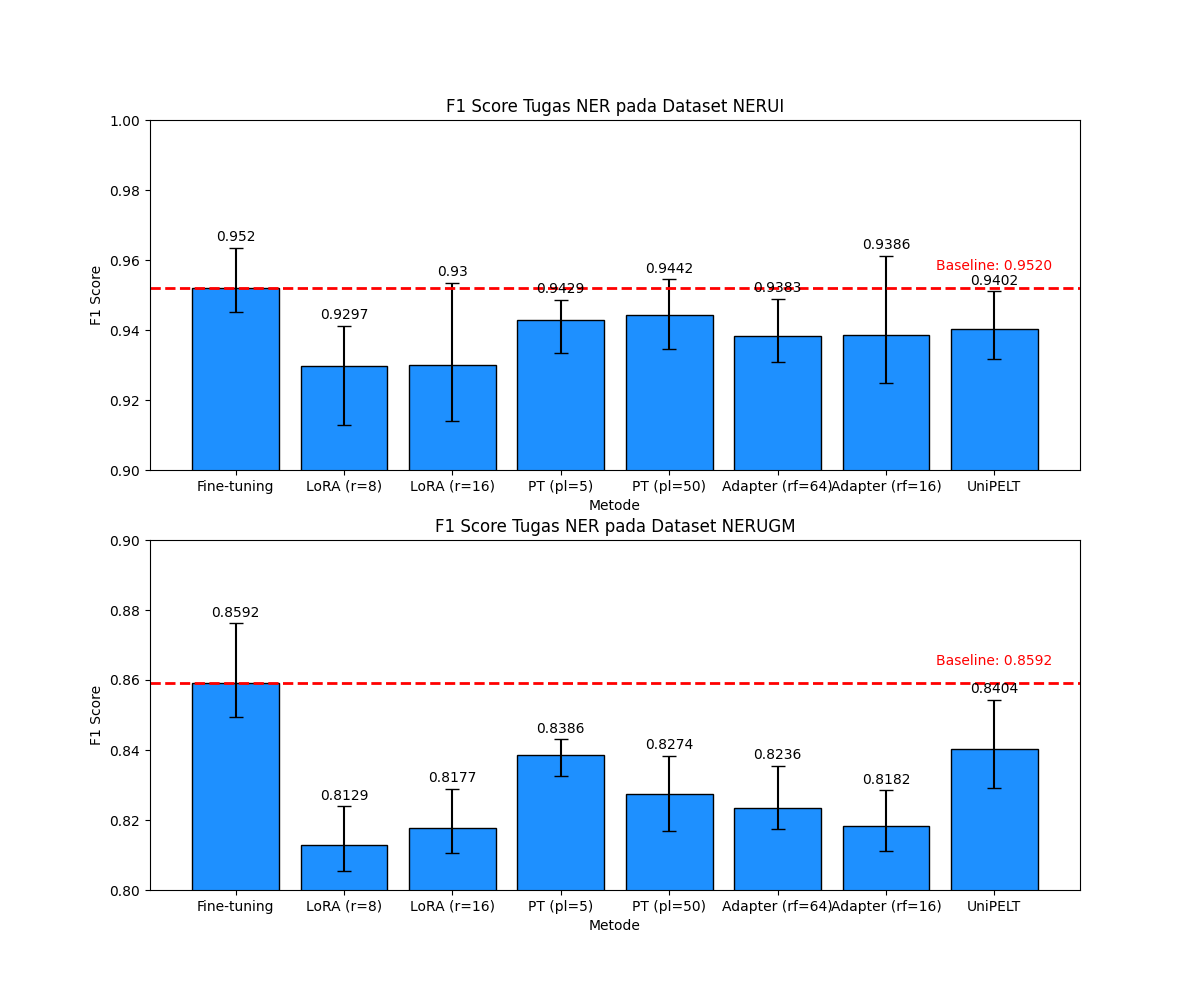
\includegraphics[width=1.2\textwidth]{chapter-4/ner_result.png}}
    \caption{\textit{F1 Score} Hasil Evaluasi NER}
    \label{fig:ner-result}
\end{figure}

Dari gambar \ref{fig:ner-result} didapatkan hasil evaluasi F1 skor terhadap kedua \textit{dataset}, yaitu NER UI (atas) dan NER UGM (bawah). Didapatkan skor F1 untuk \textit{fine-tuning} adalah 0,952 (NER UI) dan 0,859 (NER UGM). Untuk metode PEFT, hasil yang paling mendekati adalah \textit{Prefix-Tuning} $pl=50$ dengan skor F1-nya bernilai 0,944 (NER UI) dan UniPELT dengan skor F1-nya 0,84 (NER UGM). Perbandingan untuk \textit{dataset} NER UI antara \textit{fine-tuning} dengan PEFT terbaik (dalam konteks ini \textit{Prefix-Tuning} $pl=50$) adalah 0,952 dibanding 0,944, dengan selisih sebanyak 0,008 yang berati terdapat perbedaan sebanyak 0,84\%. Lalu, perbandingan untuk NER UGM adalah 0,859 dibanding 0,84, dengan selisih sebanyak 0,0188 yang berarti terdapat perbedaan sebanyak 2,2\%. 

Metode PEFT yang terburuk pada tugas evaluasi ini adalah LoRA $r=8$ dengan nilai 0,923 untuk NER UI dan 0,813 untuk NER UGM. Ketika dibandingkan dengan \textit{fine-tuning}, untuk NER UI adalah 0,952 dibanding 0,923 dengan selisih sebesar 3\%. Lalu, untuk NER UGM, nilainya adalah 0,859 dibanding 0,813 dengan selisih 5,4\%. Ketika ditinjau sebagai rentang persentase selisih secara keseluruhan, didapatkan rentang antara 0,84\% sampai 5,4\% untuk tugas evaluasi NER. Perbandingan yang cukup kecil mengingat dari jumlah parameter yang digunakan dan waktu pelatihannya yang lebih singkat.

Ditinjau dari konfigurasi model PEFT yang digunakan, pada hal ini adalah $rank$ untuk LoRA, $prefix\_length$ untuk \textit{Prefix-Tuning}, dan $reduction\_factor$ untuk \textit{Adapter}, hanya LoRA yang konsisten lebih baik pada kedua \textit{dataset}. \textit{Prefix-Tuning} dan \textit{Adapter} tidak konsisten berdasarkan konfigurasi pada hasil evaluasi. Untuk meninjau kinerja setiap PEFT secara setara dilakukan perbandingan dengan menggunakan konfigurasi yang terbaik untuk setiap \textit{dataset} yang bisa dilihat pada tabel \ref{table:ner-result-desc}.

\begin{table}[h]
    \centering
    \caption{Tabel skor F1 (terurut secara menurun) tugas NER dengan konfigurasi terbaik}
    \label{table:ner-result-desc}
    \begin{tabular}{ll|ll}
        \toprule
        \textbf{Metode} & \textbf{F1 NER UI $\downarrow$} & \textbf{Metode} & \textbf{F1 NER UGM $\downarrow$} \\
        \midrule
        \textit{Fine-tuning} & 0,952 & \textit{Fine-tuning} & 0,859 \\
        \textit{Prefix-Tuning} & 0,944 & UniPELT & 0,84 \\
        \textit{UniPELT} & 0,94 & \textit{Prefix-Tuning} & 0,838 \\
        \textit{Adapter} & 0,939 & \textit{Adapter} & 0,824 \\
        LoRA & 0,93 & LoRA & 0,82 \\
        \bottomrule
    \end{tabular}
\end{table}

Hasil yang didapatkan dengan menggunakan konfigurasi metode PEFT terbaik dan diurutkan secara menurun bisa dilihat pada tabel \ref{table:ner-result-desc}. Berdasarkan hasil tersebut, \textit{fine-tuning} tetap mendapatkan hasil yang terbaik, disusul oleh \textit{UniPELT} dan \textit{Prefix-Tuning} pada peringkat yang sama, \textit{Adapter}, dan LoRA pada urutan terakhir.

\subsection{Hasil Evaluasi \textit{Sentiment Analysis}}
\label{sec:sentiment-evaluation}

Evaluasi dilakukan untuk model IndoBERT dengan melakukan 8 eksperimen (\textit{fine-tuning} dan PEFT beserta variasinya) pada 5-\textit{fold dataset} untuk tugas \textit{sentiment analysis}. Berbeda dengan tugas NER yang dibahas pada subbab \ref{sec:ner-evaluation}, tugas \textit{sentiment analysis} hanya mempunyai satu \textit{dataset} yang tersedia pada kakas evaluasi IndoLEM. Hasil evaluasi yang didapatkan merupakan waktu pelatihan dan juga skor F1 dari data evaluasi, hasil tersebut bisa dilihat pada tabel \ref{table:runtime-sentiment} dan gambar \ref{fig:ner-result}. Sama seperti subbab \ref{sec:ner-evaluation}, skor F1 dan waktu pelatihan merupakan hasil dari rata-rata pada seluruh 5-\textit{fold}.

\begin{table}[h]
    \centering
    \caption{Waktu pelatihan tugas \textit{sentiment analysis}}
    \label{table:runtime-sentiment}
    \begin{tabular}{l|rr}
        \toprule
        \textbf{Metode} & \textbf{Waktu(s) \%} \\
        \midrule
        \textit{Fine-tuning} & \textcolor{Red}{866 (100\%)} \\
        LoRA ($r$=8) & 627 (72\%) \\
        LoRA ($r$=16) & 627 (72\%) \\
        Prefix Tuning ($pl$=5) & 619 (72\%) \\
        Prefix Tuning ($pl$=50) & 652 (75\%) \\
        Adapter ($rf$=64) & \textcolor{Green}{613 (71\%)} \\
        Adapter ($rf$=16) & 617 (71\%) \\
        UniPELT & 746 (86\%) \\
        \bottomrule
    \end{tabular}
\end{table}

Dari tabel \ref{table:runtime-sentiment}, didapatkan waktu pelatihan yang paling cepat adalah \textit{Adapter} $rf=64$ dengan waktu yang dibutuhkan sebanyak 613 detik, sebaliknya waktu pelatihan yang paling lambat adalah \textit{fine-tuning} dengan waktu sebesar 866 detik. Perbandingan antara waktu pelatihan yang tercepat yaitu \textit{Adapter} $rf=64$ dengan perbandingan sebesar 71\% dibandingkan dengan waktu pelatihan pada \textit{fine-tuning}. Untuk tugas evaluasi \textit{sentiment analysis}, setiap metode PEFT berhasil mendapatkan waktu pelatihan yang lebih cepat dibandingkan dengan \textit{fine-tuning}. Rentang perbandingan waktu yang dibutuhkan dibandingkan dengan \textit{fine-tuning} adalah antara 71\% (\textit{Adapter}) sampai 86\% (UniPELT). Rasio dari waktu pelatihan yang didapatkan sesuai dengan pada penelitian yang dilakukan oleh \citeauthor{unipelt}, bisa dilihat pada tabel \ref{table:unipelt_result}.

\begin{figure}[h]
    \centering
    \centerline{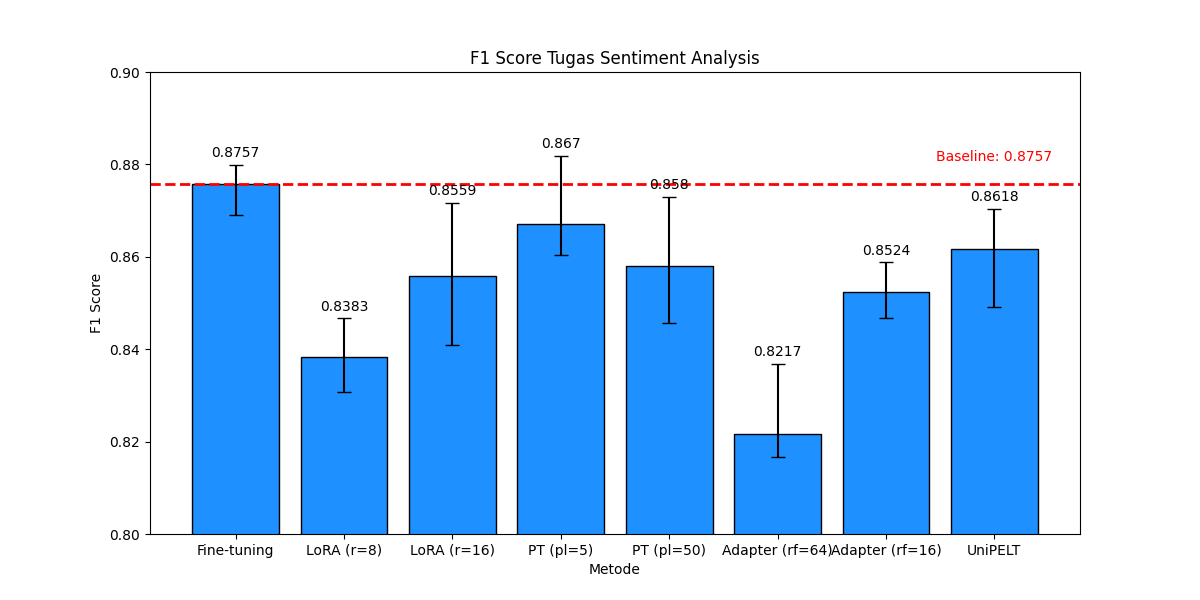
\includegraphics[width=1.2\textwidth]{chapter-4/sentiment_result.png}}
    \caption{\textit{F1 Score} Hasil Evaluasi \textit{Sentiment Analysis}}
    \label{fig:sentiment-result}
\end{figure}

Berdasarkan skor F1 pada gambar \ref{fig:sentiment-result}, \textit{fine-tuning} mendapatkan skor yang terbaik dengan nilai 0,876 disusul oleh metode \textit{Prefix-Tuning} $pl=5$ dengan nilai 0,867. Selisih yang didapatkan antara \textit{fine-tuning} dengan metode PEFT terbaik (\textit{Prefix-Tuning} $pl=5$) adalah 0,876 dibanding 0,867, dengan nilai selisihnya yaitu 0,009 atau sekitar 1\%. Sedangkan, untuk metode PEFT terburuk secara skor F1 adalah 0,822 yaitu metode \textit{Adapter} $rf=64$. Dibandingkan antara \textit{fine-tuning} dengan \textit{Adapter} $rf=64$ yaitu 0,822 dibanding 0,876 dengan selisihnya sebesar 0,054 atau sekitar 6,2\%. Demikian didapatkan rentang selisih untuk semua metode PEFT dibandingkan dengan \textit{fine-tuning} adalah antara 1\% sampai 6,2\%. Perbandingan ini terhitung cukup kecil jika mengingat penggunaan parameter pelatihan dan waktu pelatihan yang lebih sedikit. Sehingga, terdapat \textit{tradeoff} antara parameter pelatihan yang lebih kecil dan waktu pelatihan yang lebih cepat dengan hasil evaluasi yang lebih buruk.

Pada tugas evaluasi ini, konfigurasi untuk metode PEFT konsisten lebih baik untuk parameter yang lebih banyak untuk LoRA dan \textit{Adapter}. LoRA dengan $r=16$ mendapatkan hasil yang lebih baik dibandingkan dengan $r=8$. Begitu juga dengan \textit{Adapter} dengan $rf=16$ mendapatkan hasil yang lebih baik dibanding $rf=64$ ($rf$ merupakan faktor reduksi, sehingga $rf$ yang lebih kecil akan menghasilkan parameter yang lebih banyak). Tetapi, hal yang sebaliknya terjadi untuk metode \textit{Prefix-Tuning}, variasi $pl=5$ ternyata menghasilkan skor F1 yang lebih baik dibandingkan dengan $pl=50$. Untuk meninjau kinerja metode PEFT secara dilakukan perbandingan dengan skor F1 berdasarkan hasil yang paling baik untuk setiap variasinya.

\begin{table}[h]
    \centering
    \caption{Tabel F1 (terurut secara menurun) tugas \textit{sentiment analysis} dengan konfigurasi terbaik}
    \label{table:sentiment-result-desc}
    \begin{tabular}{l|l}
        \toprule
        \textbf{Metode} & \textbf{F1 $\downarrow$} \\
        \midrule
        \textit{Fine-tuning} & 0,876 \\
        \textit{Prefix-tuning} & 0,867 \\
        \textit{UniPELT} & 0,862 \\
        \textit{LoRA} & 0,856 \\
        \textit{Adapter} & 0,852 \\
        \bottomrule
    \end{tabular}
\end{table}

Tabel \ref{table:sentiment-result-desc} menunjukkan skor F1 yang terurut secara menurun untuk metode PEFT dengan konfigurasi terbaik. \textit{Fine-tuning} mendapatkan hasil yang paling baik, disusul oleh \textit{Prefix-Tuning}, UniPELT, LoRA, lalu Adapter. Urutan ini cukup konsisten dengan untuk tugas NER pada tabel \ref{table:ner-result-desc}. Namun, terdapat perbedaan untuk metode PEFT pada urutan terakhir, pada tugas evaluasi ini, urutan terakhir dipegang oleh \textit{Adapter}.

\subsection{Hasil Evaluasi \textit{Summarization}}

Evaluasi dilakukan untuk model IndoT5 dengan melakukan 8 eksperimen (\textit{fine-tuning} dan PEFT beserta variasinya) pada \textit{dataset} IndoSum yang tersedia pada kakas IndoLEM. Meskipun \textit{dataset} untuk tugas \textit{summarization} menggunakan 5-\text{fold cross validation}, tetapi pada eksperimen ini tidak dilakukan untuk 5\textit{-fold}, hanya dilakukan pada \textit{fold} pertama saja karena kerterbatasan sumber daya. Hasil evaluasi yang didapatkan berupa waktu pelatihan dan skor ROUGE (R1, R2, dan RL) dari data evaluasi, hasil tersebut bisa dilihat pada tabel \ref{table:runtime-summarization-indosum} dan gambar \ref{fig:summarization-result-indosum}.

\begin{table}[h]
    \centering
    \caption{Waktu pelatihan tugas \textit{summarization} IndoSum}
    \label{table:runtime-summarization-indosum}
    \begin{tabular}{l|r}
        \toprule
        \textbf{Metode} & \textbf{Waktu(s) \%} \\
        \midrule
        \textit{Fine-tuning} & 5026 (100\%) \\
        LoRA ($r$=8) & 4841 (96\%) \\
        LoRA ($r$=16) & 4900 (97\%) \\
        Prefix Tuning ($pl$=5) & 6618 (132\%) \\
        Prefix Tuning ($pl$=50) & \textcolor{Red}{11379 (227\%)} \\
        Adapter ($factor$=64) & \textcolor{Green}{4578 (91\%)} \\
        Adapter ($factor$=16) & 4587 (91\%) \\
        UniPELT & 9241 (184\%) \\
        \bottomrule
    \end{tabular}
\end{table}

Dari waktu pelatihan yang didapatkan dari tabel \ref{table:runtime-summarization-indosum}, terdapat waktu pelatihan tercepat adalah \textit{Adapter} $rf=64$ dengan waktu sebesar 4,578 detik. Untuk waktu pelatihan yang terlambat adalah \textit{Prefix-Tuning} $pl=50$ dengan waktu sebesar 11,379 detik. Jika dibandingkan dengan \textit{fine-tuning}, waktu tercepat menggunakan 91\% dari waktu pelatihan, hal ini berbeda dari subbab \ref{sec:ner-evaluation} dan \ref{sec:sentiment-evaluation} yang bisa mendapatkan hasil lebih cepat. Selain itu, untuk waktupaling lambat didapatkan perbandingan sebesar 227\%, yang berarti waktu pelatihannya lebih dari 2 kali lipat dibanding \textit{fine-tuning}. Metode \textit{Prefix-Tuning} dan UniPELT membutuhkan waktu pelatihan yang lebih dari \textit{fine-tuning} ($>100\%$). 

Untuk memastikan perilaku ini konsisten terhadap tugas \textit{summarization}, dilakukan percobaan pada metode \textit{Prefix-Tuning} pada \textit{fold} yang berbeda. Untuk \textit{fold} yang berbeda juga didapatkan hasil yang sama, yaitu 6535 detik untuk $pl=5$ pada \textit{fold} kedua. Perilaku ini konsisten terhadap tugas \textit{summarization} pada \textit{dataset} IndoSum. Dilakukan juga eksperimen pada \textit{dataset} yang berbeda, yaitu Liputan6 secara \textit{abstractive} dan \textit{extractive}. Untuk mempersingkat eksperimen yang dilakukan, hanya digunakan sampel data sebanyak 1000 untuk setiap data latih, validasi, dan uji pada Liputan6.

\begin{table}[h]
    \centering
    \caption{Waktu pelatihan tugas \textit{summarization} Liputan6}
    \label{table:runtime-summarization-liputan6}
    \begin{tabular}{l|r|r}
        \toprule
        \multirow{2}{*}{\textbf{Metode}} & \textbf{Waktu(s)}  & \textbf{Waktu(s)}  \\
                                         & \textbf{\textit{Abstractive}} & \textbf{\textit{Extractive}} \\
        \midrule
        \textit{Fine-tuning} & 1412 (100\%) & 1485 (100\%) \\
        LoRA ($r=8$) & 1410 (100\%) & 2125 (143\%) \\
        LoRA ($r=16$) & 1512 (107\%) & 2138 (144\%) \\
        \textit{Prefix-Tuning} ($pl=5$) & 1435 (102\%) & 1610 (108\%) \\
        \textit{Prefix-Tuning} ($pl=50$) & \textcolor{Red}{4252 (301\%)} & \textcolor{Red}{6572 (443\%)} \\
        \textit{Adapter} ($rf=64$) & \textcolor{Green}{727 (51\%)} & 1265 (85\%) \\
        \textit{Adapter} ($rf=16$) & 754 (53\%) & \textcolor{Green}{1217 (82\%)} \\
        UniPELT & 4104 (291\%) & 4145 (279\%) \\
        \bottomrule
    \end{tabular}
\end{table}

Hasil yang sama juga didapatkan dengan \textit{dataset} yang berbeda, seperti yang bisa dilihat pada tabel \ref{table:runtime-summarization-liputan6}. Metode \textit{Prefix-Tuning} perlu menggunakan waktu paling lama, bahkan pada Liputan6 secara \textit{extractive} waktu pelatihan sampai 4 kali lipatnya. Untuk tugas \textit{summarization}, tidak didapatkan hasil yang konsisten antara perbandingan parameter dengan waktu pelatihannya, terutama pada metode \textit{Prefix-Tuning}. Metode LoRA dan \textit{Adapter} cukup konsiten dibandingkan dengan tugas evaluasi sebelumnya, sedangkan UniPELT terkena dampak dari gagalnya metode \textit{Prefix-Tuning}.

\begin{figure}[h]
    \centering
    \centerline{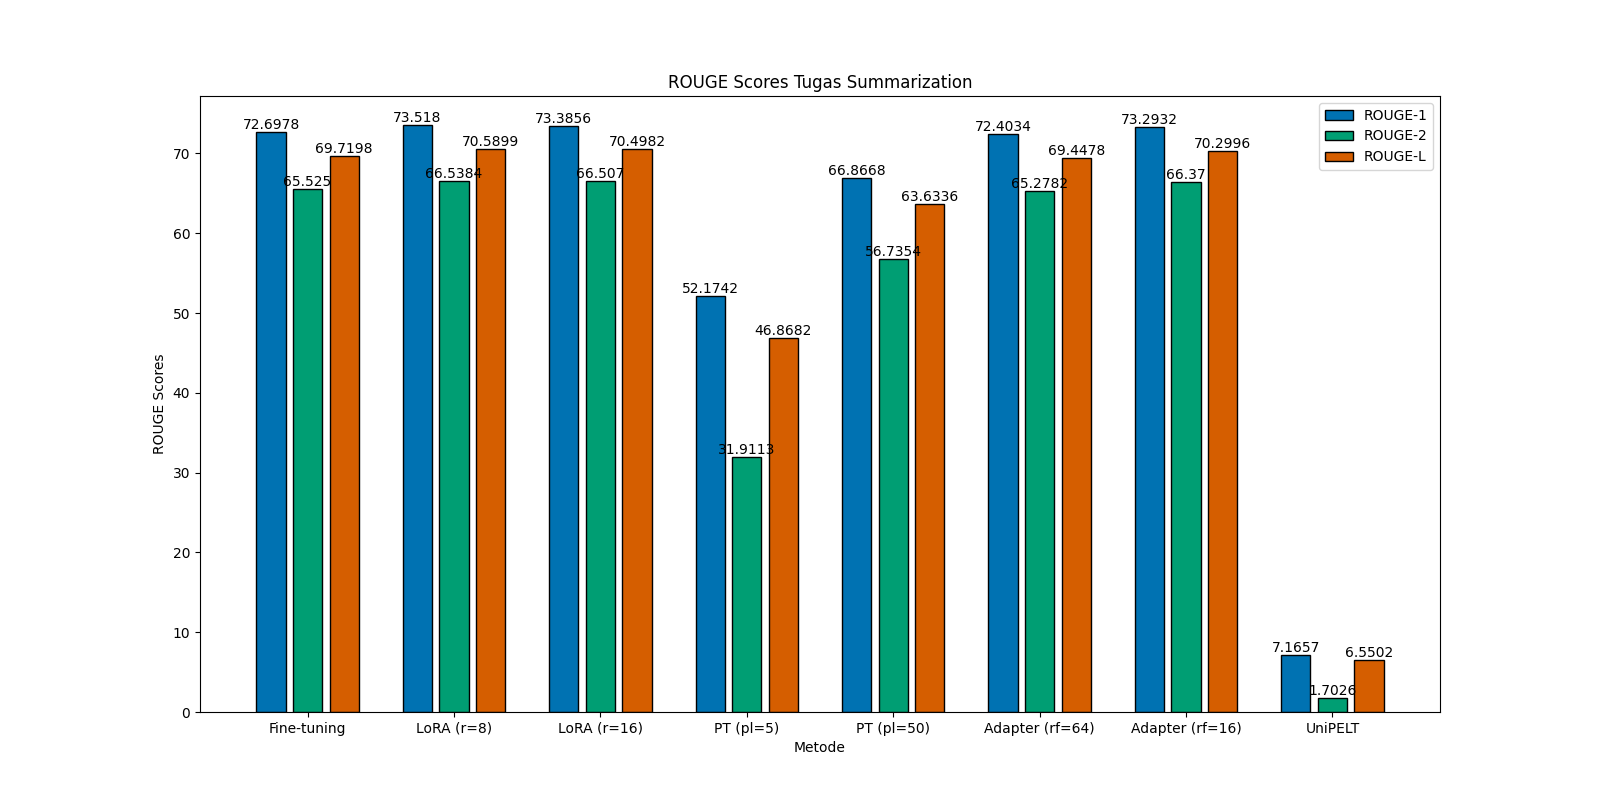
\includegraphics[width=1.4\textwidth]{chapter-4/summarization_result.png}}
    \caption{ROUGE \textit{Score} Hasil Evaluasi \textit{Summarization} pada IndoSum}
    \label{fig:summarization-result-indosum}
\end{figure}

Hasil skor ROUGE untuk \textit{dataset} IndoSum dapat dilihat pada gambar \ref{fig:summarization-result-indosum}. Terdapat tiga skor ROUGE yang digunakan yaitu R1, R2, dan RL. Secara umum, nilai dari R1 adalah yang paling tinggi untuk setiap metode, disusul oleh RL, lalu R2. Hal ini konsisten dengan perhitungan ROUGE yang menggunakan n-gram kecocokan, sehingga R1 yang mencocokan 1-gram kata secara natural akan lebih baik dibanding 2-gram dan L-gram (LCS). Skor ROUGE (ketiganya) yang paling tinggi adalah LoRA $r=8$, ini berbeda dengan tugas evaluasi sebelumnya, yang selalu didahului oleh \textit{fine-tuning}. Sedangkan, untuk nilai yang paling rendah adalah UniPELT degan skor yang sangat buruk.

Selisih yang paling signifikan adalah UniPELT dengan selisih sebesar 90\% dibandingkan dengan \textit{fine-tuning}. Namun, untuk LoRA terdapat peningkatan dengan selisih sebesar +1,25\% (simbol + menandakan peningkatan dari metode \textit{fine-tuning}). Dari selish tersebut, didapatkan rentang kinerja antara metode PEFT dengan \textit{fine-tuning} yaitu dari -90\% sampai +1,25\%. Untuk membandingkan antara metode PEFT secara setara akan dipilih variasi dari setiap PEFT dengan hasil terbaik, hasil perbandingan dapat dilihat pada tabel \ref{table:summarization-result-indosum-desc}.

\begin{table}[h]
    \centering
    \caption{Tabel ROUGE (terurut secara menurun) tugas \textit{summarization} dengan konfigurasi terbaik}
    \label{table:summarization-result-indosum-desc}
    \begin{tabular}{l|lll}
        \toprule
        \textbf{Metode} & \textbf{R1 $\downarrow$} & \textbf{R2 $\downarrow$} & \textbf{RL $\downarrow$} \\
        \midrule
        \textit{LoRA} & 73,52 & 66,54 & 70,59 \\
        \textit{Adapter} & 73,29 & 66,37 & 70,3 \\
        \textit{Fine-tuning} & 72,7 & 65,52 & 69,72 \\
        \textit{Prefix-Tuning} & 66,87 & 56,74 & 63,63 \\
        \textit{UniPELT} & 7,17 & 1,7 & 6,55 \\
        \bottomrule
    \end{tabular}
\end{table}

Berdasarkan tabel \ref{table:summarization-result-indosum-desc}, didapatkan kinerja dari masing-masing metode PEFT yang diurutkan secara menurun. Hasil yang didapatkan sangat berbeda dibanding pada tugas evaluasi NER dan \textit{sentiment analysis}, metode PEFT yaitu LoRA dan \textit{Adapter} unggul dibandingkan dengan \textit{fine-tuning}. Sedangkan, \textit{Prefix-Tuning} dan UniPELT gagal untuk menghasilkan kinerja yang menyaingi \textit{fine-tuning}. UniPELT bahkan hanya menghasilkan perbedaan kinerja sebanyak 90\% lebih buruk.

Sebelumnya, sudah disebutkan pada subbab \ref{sec:prefix-tuning} terkait \textit{Prefix-Tuning} bahwa implementasi dari metode tersebut berbeda karena sudah diadaptasi untuk tugas \textit{classification}. Selain itu, evaluasi yang dilakukan oleh \citeauthor{adapters} (yang mengajukan pustaka Adapters) tidak terdapat tugas evaluasi untuk tugas \textit{generation}. Evaluasi juga menggunakan model RoBERTa yang merupakan variasi dari BERT (\textit{encoder}). Sehingga, memungkinkan bahwa metode \textit{Prefix-Tuning} yang digunakan pada eksperimen ini (tugas \textit{generation} dan model \textit{encoder decoder}) tidak sesuai dengan implementasi dari modul Adapters. Hal ini menyebabkan gagalnya metode \textit{Prefix-Tuning}, yang secara langsung berkaitan juga dengan kegagalan dari UniPELT.

